% !TEX root =  paper.tex
\section{Biologically-Constrained Region Merging}

Automatic reconstruction methods need to be fast enough to scale to petabyte datasets while still maintaining a high-level of accuracy.
The most accurate methods, like flood-filling networks~\cite{januszewski2016flood}, are currently far too slow.
Unfortunately, methods that can scale to petabyte datasets typically rely on only local context and can produce errors at scale~\cite{haehn2017scalable}. 
Therefore, it is necessary to employ error correction strategies on the segmentations from current reconstruction pipelines.
We propose a biologically-constrained region merging algorithm to correct \textit{split errors} in the initial segmentation.

\subsection{Related Works}

A significant amount of connectomics research considers the problem of extracting segmentation information at the voxel level of EM images.
First, intermediate representations like boundary, affinity or binary segmentation maps are generated from the voxels.
Random forests with hand-designed features~\cite{kaynig2015large}, or 2D and 3D convolutional networks produce boundary probabilities~\cite{bogovic2013learned,ciresan2012deep,jain2010boundary,seymour2016rhoananet,ronneberger2015u,amelio_segmentation}.
Often, the affinity between each voxel and its six neighbors are used~\cite{cciccek20163d,lee2015recursive,lee2017superhuman,parag2017anisotropic,turaga2010convolutional}. 
The 3D U-Net architecture has become popular~\cite{cciccek20163d} and the MALIS cost function is specifically designed to re-weight affinity predictions by their contribution to the segmentation error~\cite{briggman2009maximin}.
More recently, flood-filling networks~\cite{januszewski2016flood} produce binary segmentations from raw pixels with a recurrent convolutional network at a high computational cost.
Orthogonal to the representation, model averaging~\cite{zeng2017deepem3d} and data augmentation~\cite{lee2017superhuman} methods can further improve the performance, where Lee et al.~\cite{lee2017superhuman} surpass the estimated human accuracy on the SNEMI3D dataset.

Clustering techniques transform these intermediate representations into segmentations.
Some early methods apply computationally expensive graph partitioning algorithms with a single node per superpixel~\cite{andres2012globally}.
Several pixel-based approaches generate probabilities that neighboring pixels belong to the same neuron.
Often a watershed algorithm will then cluster these pixels into super-pixels~\cite{zlateski2015image}.

Region merging methods can be categorized by the similarity metric between adjacent segments and the merging strategy.
For the similarity metric, Lee et al. and Funke et al. rely solely on the accuracy of the predicted affinities and define the metric as the mean affinity between segments~\cite{funke2017deep,lee2017superhuman}.
Classification-based methods generate the probability to merge two segments from handcrafted~\cite{jain2011learning,seymour2016rhoananet,nunez2014graph,10.1371/journal.pone.0125825,parag2017anisotropic,zlateski2015image} and learned features~\cite{bogovic2013learned}. 
For the merging strategy, most methods use variants of hierarchical agglomeration ~\cite{seymour2016rhoananet,nunez2014graph,10.1371/journal.pone.0125825,parag2017anisotropic,zlateski2015image} to greedily merge a pair of regions at a time.
Jain et al. formulates the agglomeration problem as a reinforcement learning problem ~\cite{jain2011learning} and Pape et al. present a scalable multicut algorithm to partition superpixels with global optimization~\cite{beier2017multicut}.

Additional research builds on top of these region-based methods to correct errors in the segmentation. 
These input segmentations can contain two types of errors.
In a \textit{split error}, one neuron contains multiple labels.
In a \textit{merge error}, two or more neurons receive the same label.
This can be done either using human proofreading~\cite{haehn2017guided,haehn2014design,mojo2} or automatically~\cite{rolnick2017morphological,error_correction_using_CNN}. 
In both cases, available methods are pixel-based and do not include global biological constraints into the decision making process. 
Our method can take as input any existing segmentation pipeline.

\subsection{Method}

\begin{figure*}[t!]
	\centering
	\includegraphics[width=0.65\linewidth]{./figures/teaser_v4.png}
	\caption{Our framework uses both geometric and topological biological constraints for region merging. We (a) generate a simplified graph from the skeleton representation of the input segmentation, (b) train a classifier to learn the edge weight based on the shape of the segment connection, and (c) perform graph partitioning with acyclic constraints.}
	\label{fig:teaser_pipeline}
\end{figure*}


For our proposed method (Fig.~\ref{fig:teaser_pipeline}), from the input segmentation we generate a graph $G$ with nodes $N$ and edges $E$ with weights $w_e$. 
The nodes correspond to labeled segments from the input data with edges between merge candidates.
We propose the following three steps to formulate and then partition the graph while obeying constraints from the underlying biology.
First, we only consider merging segments based on a skeletonized representation of the input segmentation (Fig.~\ref{fig:teaser_pipeline}a).
This enables us to reduce the number of edges in the graph based on prior knowledge on the shape of neuronal processes.
Second, we train a convolutional neural network that learns biological constraints based on the shapes of the input segmentation (Fig.~\ref{fig:teaser_pipeline}b).
This network generates probabilities that segments belong to the same neuron based only on the segmentations. 
An example of one such learned constraint is that neurons have small turning radii (Fig.~\ref{fig:turn-radii}).
Third, we partition the graph using a lifted multicut formulation with additional acyclic constraints to enforce global biological constraints (Fig.~\ref{fig:teaser_pipeline}c).
The lifted multicut solution is globally consistent which we then augment to produce a tree-structured graph.


\begin{figure}[t]
	\centering
	\begin{minipage}{0.45\linewidth}
		\includegraphics[width=\linewidth]{./figures/skeleton1.png}		
	\end{minipage}
	\hfill
	\begin{minipage}{0.45\linewidth}
		\includegraphics[width=\linewidth]{./figures/skeleton2.png}		
	\end{minipage}
	\begin{minipage}{0.45\linewidth}
		\includegraphics[width=\linewidth]{./figures/skeleton3.png}		
	\end{minipage}
	\hfill
	\begin{minipage}{0.45\linewidth}
		\includegraphics[width=\linewidth]{./figures/skeleton4.png}		
	\end{minipage}
	\caption{Example skeletons (in black) extracted from segments using a variant of the TEASER algorithm~\cite{sato2000teasar}. These skeletons not only capture the shape of the segmentation, but also provide endpoints useful for region merging proposals.}
	\label{fig:skeletonization}
\end{figure}

\subsubsection{Skeleton-Based Graph Generation}
\label{sec:skeletonization}

Most region merging methods create a region graph by removing small-sized segments and linking each pair of adjacent segments, which can still lead to a large graph size due to the irregular shape of neural structures.
We use a skeleton representation of the segmentation to reduce the graph size with geometric constraints on the connectivity of two adjacent segments to prune edges.

Our key observation is that if two segments belong to the same neuronal process, their skeleton end points should satisfy certain geometric constraints.
To extract the skeleton from each segment, we use a variant~\cite{zhao2014automatic} of the TEASER algorithm~\cite{sato2000teasar}. 
Fig.~\ref{fig:skeletonization} shows four examples of extracted skeletons (in black). 
These skeletons consist of a sequence of \textit{joints}, locations that are locally a maximum distance from the segment boundary, with line segments connecting successive joints. 
We refer to joints that have only one connected neighbor as \textit{endpoints}. 
We find that approximately 70\% of the segments that are erroneously split have nearby endpoints (Fig.~\ref{fig:merge_candidates}). 

Two segments, $s_1$ and $s_2$, receive a corresponding edge if the two following conditions hold.
First, endpoints in either $s_1$ or $s_2$ are within $t_{low}$ nm of any voxel in the other segment.
Second, there are endpoints in $s_1$ and in $s_2$ that are within $t_{high}$ nm of each other.
We store the midpoints between the two endpoints as the center of the potential merge in the set $\mathbb{S}_c$. 
This algorithm produces a set of segments to consider for merging. 
Only these pairs have a corresponding edge in the constructed graph.

\subsubsection{Learning-based Edge Weight}
\label{sec:edge-weights}

To predict the probabilities that two segments belong to the same neuron, we train a feed-forward convolutional network with three \textit{VGG-style} convolution blocks~\cite{chatfield2014return} and two fully connected layers before the final sigmoid activation. 
For the input of the network, we extract a cubic region of interest (ROI) around each midpoint in $\mathbb{S}_c$ as input to the CNN. 
There are three channels corresponding to voxels belonging to label one, label two, or either label.
We do not use the raw EM image information to avoid the need to retrain the network on datasets that have been stained differently or imaged at different resolution. 
This reduces the need for generating costly manually-labeled ground truth. 
\begin{figure}[t]
	\begin{minipage}{0.4\linewidth}
		\includegraphics[width=\linewidth]{./figures/constraint_error.png}
	\end{minipage}
	\hfill
	\begin{minipage}{0.55\linewidth}
		\includegraphics[width=\linewidth]{./figures/constraint_success.png}
	\end{minipage}
	\caption{Geometric constraints for region merging. We show two region merging proposals. On the left, the segments do not belong to the same neuron, as evidenced by the sharp turning radius indicated by the arrow; while on the right, the segments should be merged due to the continuity of the 3D shape. Instead of using handcrafted geometric features, we train a convolutional neural networks to automatically learn them from the ground truth labels.}
	\label{fig:turn-radii}
\end{figure}

\subsubsection{Optimization-Based Graph Partition}

\label{sec:optimization}

After constructing the graph we seek to partition it into labels where every label corresponds to a neuronal process. 
We formulate this graph partitioning problem as a multicut problem.
There are two primary benefits to using a multicut formulation. 
First, the number of segments in the final graph is not predetermined but depends on the input. 
Second, this minimization produces globally consistent solutions (i.e., a boundary remains only if the two corresponding nodes belong to unique segments)~\cite{keuper2015efficient}.

We apply the algorithms of Keuper et al.~\cite{keuper2015efficient} to produce a feasible solution to the multicut problem using greedy additive edge contraction.
Following their example, we employ the generalized lifted multicut formulation.
Traditional multicut solutions only consider the probabilities that two adjacent nodes belong to the same segment. 
In the lifted extension to the problem, we can penalize non-adjacent nodes that belong to different segments. 
These penalties between non-adjacent nodes are called lifted edges. 
Ideally these lifted weights represent the probability that two nodes belong to the same neuron.
However, determining such probabilities is computationally expensive.
We approximate these probabilities by finding the maximal probable path between any two nodes using Dijkstra's algorithm~\cite{keuper2015efficient}.
This is an underestimate of the probability that two nodes belong to the same neuron since it does not consider all possible paths.
Since our graphs are sufficiently small, we can generate lifted edges between all pairs of nodes. 

We need to convert the probabilities into the following weighting scheme to solve the multicut problem with the greedy-edge heuristic~\cite{andres2011probabilistic,keuper2015efficient}.
Given the probability that the nodes belong to the same neuron is $p_e$, the edge weight $w_e$ is defined as
%p_e &=\mbox{CNN}(x_1, x_2) \\
\begin{align}
w_e = \log{\frac{p_e}{1 - p_e}} + \log{\frac{1 - \beta}{\beta}},
\end{align}
where $\beta$ is a tunable parameter that encourages over or undersegmentation. 
Since, there are many more lifted edges than adjacent edges, we scale down the lifted weights proportionally to their total number  
~\cite{beier2017multicut}.

By reformulating the segmentation problem as a graph partitioning one, we can enforce some global constraints on our result based on the underlying biology.
Traditional hierarchical clustering algorithms do not rely on such constraints but consider local decisions independently.
We enforce a global constraint that neurons are tree-structured and should not contain cycles. 
The multicut problems returns a series of ``collapsed'' edges between nodes that belong to the same neuron.
We iterate over these edges in order of the probability of merge generated by our CNN. 
We ``collapse'' an edge only if it does not create a cycle in the graph.

\begin{figure}[t]
	\centering
	\begin{minipage}{0.32\linewidth}
		\includegraphics[width=\linewidth]{./figures/split_error1.png}		
	\end{minipage}
	\hfill
	\begin{minipage}{0.32\linewidth}
		\includegraphics[width=\linewidth]{./figures/split_error2.png}				
	\end{minipage}
	\hfill
	\begin{minipage}{0.32\linewidth}
		\includegraphics[width=\linewidth]{./figures/split_error3.png}
	\end{minipage}
	\caption{Three erroneously split segments. In each instance, the skeletons for each segment have nearby endpoints indicating a split error.}
	\label{fig:merge_candidates}
\end{figure}


\subsection{Experiments}

We evaluate our method by comparing it to a state-of-the-art pixel-based reconstruction approach using datasets from mouse and fly brains.

\subsubsection{Datasets}
\label{sec:dataset}

Our first dataset, which we call the Kasthuri dataset, consists of scanning electron microscope images of the neocortex of a mouse brain~\cite{kasthuri2015saturated}. 
This dataset is $5342 \times 3618 \times 338$ voxels in size. 
The resolution of the dataset is $\SI[product-units=single]{3 x 3 x 30}{\nano\meter}^3$ per voxel. 
We divide the dataset into two volumes (Vol. 1 and Vol. 2) along the $x$ dimension, where each volume is $\SI[product-units=single]{8.0 x 10.9 x 10.1}{\micro\meter}^3$.
We train and validate our methods on Vol. 1 and test on Vol. 2.
Our second dataset, called FlyEM, comes from the mushroom body of a 5-day old adult male \textit{Drosophila} fly imaged by a focused ion-beam milling scanning electron microscopy~\cite{takemura2017connectome}.
The original dataset contains a $\SI[product-units=single]{40 x 50 x 120}{\micro\meter}^3$ volume with a resolution of $\SI[product-units=single]{10 x 10 x 10}{\nano\meter}^3$ per voxel. 
We use two cubes (Vol. 1 and Vol. 2) of size $\SI[product-units=single]{10 x 10 x 10}{\micro\meter}^3$.


\subsubsection{Method Configuration}

\noindent\textbf{Input Segmentation}
The segmentation of the Kasthuri dataset is computed by agglomerating 3D supervoxels produced by the z-watershed algorithm from 3D affinity predictions~\cite{zlateski2015image}. 
We learn 3D affinities using MALIS loss with a U-Net~\cite{ronneberger2015u,Turaga:2009}. 
We apply the z-watershed algorithm with suitable parameters to compute a 3D over-segmentation of the volume. 
The resulting 3D oversegmentation is then agglomerated using the technique of context-aware delayed agglomeration to generate the final segmentation~\cite{10.1371/journal.pone.0125825}.

For the FlyEM data, based on the authors' suggestion~\cite{takemura2017connectome}, we apply a context-aware delayed agglomeration algorithm~\cite{10.1371/journal.pone.0125825} that shows improved performance on this dataset over the pipeline used in the original publication. 
This segmentation framework learns voxel and supervoxel classifiers with an emphasis to minimize undersegmentation error. 
The algorithm first computes multi-channel 3D predictions for membranes, cell interiors, and mitochondria, among other cell features. 
The membrane prediction channel is used to produce an oversegmented volume using 3D watershed, which is then agglomerated hierarchically up to a certain confidence threshold. 
We used exactly the same parameters as the publicly available code for this algorithm.
\\~\\
\noindent\textbf{Graph Generation}
The two parameters for the graph pruning algorithm (Sec.~\ref{sec:skeletonization}) are $t_{low}$ and $t_{high}$. 
Ideally, our graph will have an edge for every oversegmented pair of labels with few edges between correctly segmented pairs. 
After considering various thresholds, we find that $t_{low} = \SI{210}{\nano\meter}$ and $t_{high} = \SI{300}{\nano\meter}$ produce expressive graphs with a scalable number of nodes and edges.
During implementation, we use nanometers instead of voxels to standardize units across all datasets.
\\~\\
\noindent\textbf{Edge Weight Learning}
\label{sec:network-parameters}
We use half of the Kasthuri dataset for training and validation. 
We train on 80\% of the potential merge candidates for this volume.
We validate the CNN classifier on the remaining 20\% of the candidates. 
Since our input does not require the image data, we can train on the anisotropic Kasthuri data and test on the isotropic FlyEM data.

\noindent\textbf{Training Augmentation}
Since our input is an existing segmentation of the EM images, there are very few training examples compared to per-pixel classifiers that train on a unique window for each voxel. 
The Kasthuri dataset represents a region of brain over $\SI[product-units=single]{800}{\micro\meter}^3$ in volume and only yields 640 positive merge examples and 4821 negative ones.
To avoid overfitting our deep networks, we apply the following augmentations on the training examples.
During a single batch, we randomly select ten positive and ten negative examples. 
With probability 0.5, an example is reflected across the $xy$-plane. 
We then rotate each example by a random angle between $0$ and $360$ degrees using nearest neighbor interpolation. 
We have 20,000 such examples per epoch.

\subsubsection{Error Metrics}
\label{sec:variation-of-information}
We evaluate the performance of the different methods using the split variation of information (VI) score~\cite{meila2003comparing}.
Given a ground truth labeling $GT$ and our automatically reconstructed segmentation $SG$, over and undersegmentation are quantified by the conditional entropies $H(GT | SG)$ and $H(SG | GT)$, respectively. 
Since we are measuring the entropy between two clusterings, lower VI scores are better.
The sum of these conditional entropies gives the total variation of information.

We use precision and recall to evaluate the convolutional neural network and multicut outputs. 
Since our method only corrects \textit{split errors}, we define a true positive as a pair of segments that are correctly merged together after our pipeline.



\begin{figure*}[t!]
	\centering
	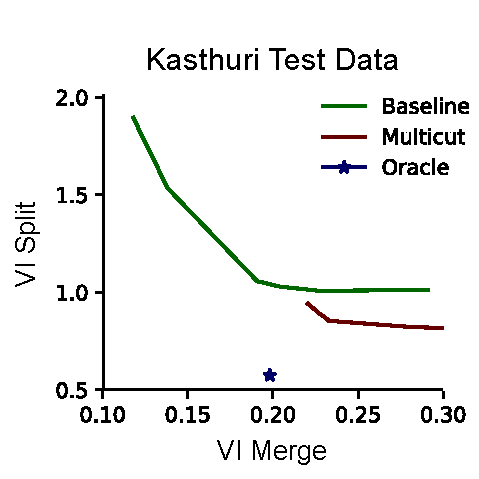
\includegraphics[width=0.32\linewidth]{./figures/benchmark/voi-Kasthuri-Luigi-Test.pdf}
	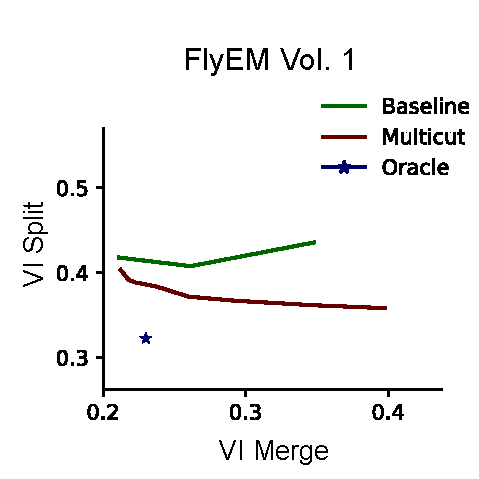
\includegraphics[width=0.32\linewidth]{./figures/benchmark/voi-FlyEM-Vol--1.pdf}
	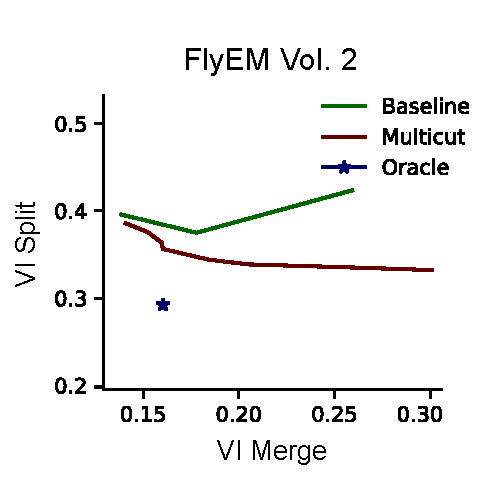
\includegraphics[width=0.32\linewidth]{./figures/benchmark/voi-FlyEM-Vol--2.pdf}
	\caption{Segmentation benchmark results on three volumes. We compare our method (red) to the baseline segmentation (green) and an oracle (blue) that optimally partitions our constructed graph from our method. Lower VI scores are better. Our method improves the segmentation accuracy over the baseline in all cases.
		Note that our model is only trained on the Kasthuri training volume and it generalizes well to the FlyEM datasets.}
	\label{fig:variation-of-information}
\end{figure*}


\subsection{Results}


In Fig.~\ref{fig:variation-of-information}, we show the VI results of the pixel-based reconstructions of the Kasthuri and FlyEM data (Sec.~\ref{sec:dataset}) for varying thresholds of agglomeration (green). 
We show comparisons to an oracle (blue) that correctly partitions the graph from our method based on ground truth.
Scores closer to the origin are better for this metric, and in every instance our results (red) are below the green curve.
We see improvements on each data with a reduction in total VI score of $10.4\%$ on the Kasthuri data and $8.9\%$ and $5.4\%$ on the FlyEM datasets.

Fig.~\ref{fig:qualitative-results} (left) shows successful merges on the Kasthuri dataset. 
Several of these examples combine multiple consecutive segments that span the volume.
In the third example on the left we correct the over-segmentation of a dendrite and attached spine-necks.
Fig.~\ref{fig:qualitative-results} (right) shows typical failure cases of our method (red circles).
In two of these examples the algorithm correctly predicts several merges before a single error renders the segment as wrong.
In the third example (blue circle) a merge error in the initial segmentation propagates to our output.
We now analyze how each major component of our method contributes to this final result.

\subsubsection{Empirical Ablation Studies}

\noindent\textbf{Graph Generation}
Table \ref{table:skeletonization} shows the results of pruning the skeleton graph using the algorithm discussed in Sec.~\ref{sec:skeletonization}. 
This edge pruning is essential for the graph partitioning algorithm, which has a non-linear computational complexity dependence on the number of edges. 
The baseline algorithm considers all adjacent regions for merging. 
Our method removes a significant portion of these candidates while maintaining a large number of the true merge locations (e.g., 764 compared to 974). 
Our pruning heuristic removes at least $3.5\times$ the number of edges on all datasets, achieving a maximum removal rate of $4.15\times$.
However, there are some adjacent oversegmented labels which are not considered. 

\begin{table*}
	\caption{The results of our graph pruning approach compared to the baseline graph with all adjacent regions. We show the number of true merge locations (e.g., 974) compared to total number of edges in the graph (e.g., 25,798) for each case. The number of missed splits corresponds to the number of split errors that our method misses compared to an adjacency matrix.}
	\resizebox{0.75\linewidth}{!}{
		\begin{tabular}{c c c c c} \hline
			\textbf{Dataset} & \textbf{Segment Adjacency} & \textbf{Skeleton Pruning} & \textbf{Missed Splits} & \textbf{Gained Edges} \\ \hline
			Kasthuri & 974 / 25,798 & 764 / 6,218 & 307 & 97 \\
			FlyEM Vol. 1 & 304 / 15,949 & 212 / 4,578 & 105 & 13 \\
			FlyEM Vol. 2 &  298 / 17,614 & 197 / 4,366 & 120 & 19 \\ \hline
		\end{tabular}
	}
	\centering
	\label{table:skeletonization}
\end{table*}

\begin{figure}[t]
	\begin{minipage}{0.45\linewidth}
		\centering
		\includegraphics[width=0.85\linewidth]{./figures/VI-results/multicut-correct1.png}
		\includegraphics[width=0.85\linewidth]{./figures/VI-results/multicut-correct2.png}
		\includegraphics[width=0.85\linewidth]{./figures/VI-results/multicut-correct3.png}
		\includegraphics[width=0.85\linewidth]{./figures/VI-results/multicut-correct4.png}
		\includegraphics[width=0.85\linewidth]{./figures/VI-results/multicut-correct5.png}
	\end{minipage}
	\begin{minipage}{0.45\linewidth}
		\centering
		\includegraphics[width=0.85\linewidth]{./figures/VI-results/multicut-incorrect1.png}
		\includegraphics[width=0.85\linewidth]{./figures/VI-results/multicut-incorrect2.png}
		\includegraphics[width=0.85\linewidth]{./figures/VI-results/multicut-incorrect3.png}
		\includegraphics[width=0.85\linewidth]{./figures/VI-results/multicut-incorrect4.png}
	\end{minipage}
	\caption{(left) Segments of neurons before they were correctly merged by our method. (right) Circles indicate areas of wrong merges by our method (red) or by the initial pixel-based segmentation (blue).}
	\label{fig:qualitative-results}
\end{figure}

We generate edges in our graph by using information from the skeletons. 
In particular, we do not enforce the constraint that edges in our graph correspond to adjacent segments.
Although neurons are continuous, the EM images often have noisy spots which cause an interruption in the input segmentation.
We still want to reconstruct these neurons despite the fact that the initial segmentation is non-continuous. 
The second and fourth examples in Fig.~\ref{fig:qualitative-results} show correctly reconstructed neurons where two of the segments are non-adjacent. 
\\~\\
\noindent\textbf{Failure Cases}
There are some pairs of segments which we do not consider for merging because of our reliance on the skeletons.
Fig.~\ref{fig:skeleton-results}, top, shows two such cases with the closest endpoints circled. 
In the right example the small segment is carved from the larger segment in a location where there are no skeleton endpoints. 
There are on average 177 such examples in our datasets.
\\~\\
\noindent\textbf{Edge Weight Learning}
Fig.~\ref{fig:receiver-operating-characteristic} shows the receiver operating characteristic (ROC) curve of our CNN classifier for all test datasets.
As shown by the ROC curve, the test results on the FlyEM data are better than the results for Kasthuri.
In part this comes from the disparity in the number of positive to negative merge candidates in the two graphs. 
The network easily classifies most of the negative examples leaving only a few difficult examples to predict.
Since there are more negative examples in relation to the positive examples in the FlyEM data, the ROC curve is greater.

\begin{figure}[t!]
	\centering
	\begin{minipage}{0.45\linewidth}
		\includegraphics[width=\linewidth]{./figures/merge_candidate1.png}	
	\end{minipage}
	\hfill
	\begin{minipage}{0.45\linewidth}	
		\includegraphics[width=\linewidth]{./figures/merge_candidate2.png}
	\end{minipage}
	\begin{minipage}{0.45\linewidth}
		\includegraphics[width=\linewidth]{./figures/merge_candidate3.png}
	\end{minipage}
	\begin{minipage}{0.45\linewidth}
		\includegraphics[width=\linewidth]{./figures/merge_candidate4.png}
	\end{minipage}
	\caption{The top two examples correspond to segment pairs that we incorrectly prune from the graph. The distance between the circled endpoints is too great. The bottom two examples show pairs of segments that belong to the same neuron but are not adjacent in the input segmentation. However, we correctly merge these pairs.}
	\label{fig:skeleton-results}
\end{figure}


%\subsection{Graph Optimization Results}
\noindent\textbf{Graph Partition}
The graph optimization strategy using multicut increases accuracy over using just the CNN.
Table \ref{table:multicut} shows the changes in precision, recall, and accuracy for all three datasets compared to the CNN with both the multicut and lifted multicut formulations.
The precision increases on each dataset, although the recall decreases on each datasets.
Since it is more difficult to correct merge errors than split errors, it is often desirable to sacrifice recall for precision.
Over the three testing datasets, applying a graph-based partitioning strategy increased the precision by $31.9\%$, $40.9\%$, and $27.8\%$ respectively. 

\begin{figure}
	\centering
	\includegraphics[width=0.9\linewidth]{./figures/receiver-operating-characteristic.png}
	\caption{The receiver operating characteristic (ROC) curves of our classifier on three connectomics datasets. The classifier works best on previously unseen data of the Kasthuri volume.}
	\label{fig:receiver-operating-characteristic}
\end{figure}

\begin{table*}[h]
	\caption{Precision, recall, and accuracy changes between CNN only and CNN paired with graph-optimized reconstructions for the training and three test datasets. The combined method results in better precision and accuracy. The lifted multicut extension provides very slight improvements in recall and accuracy over these three datasets.}
	\centering
	\resizebox{0.75\linewidth}{!}{
		\begin{tabular}{c c c c | c c c} \hline
			& \multicolumn{3}{c}{\textbf{Multicut}} & \multicolumn{3}{c}{\textbf{Lifted Multicut}} \\ \hline
			\textbf{Dataset} & $\Delta$ \textbf{Precision} & $\Delta$ \textbf{Recall} & $\Delta$ \textbf{Accuracy} & $\Delta$ \textbf{Precision} & $\Delta$ \textbf{Recall} & $\Delta$ \textbf{Accuracy} \\ \hline
			Kasthuri  & 31.94\% & -36.24\% & 0.71\% & -1.01\% & 0.60\% & 0.02\% \\
			FlyEM Vol. 1 & 40.87\% & -42.37\% & 1.26\% & 0.35\% & 0.85\% & 0.04\%  \\
			FlyEM Vol. 2 & 27.80\% & -44.95\% & 0.33\% & 0.54\% & 0.92\% & 0.04\% \\ \hline
		\end{tabular}
	}
	\label{table:multicut}
\end{table*}
